% TODO: images are on counted
\section{ЗАДАЧА МАРКЕТИНГОВОЇ РОЗВІДКИ}
% Ми не створюємо канал як такий. Метою роботи є маркетингове прогнозування 
% шляхом моделювання маркетингового каналу.
%
% TODO: можливо, заголовок треба буде змінити
% TODO: додати новий сорець
\subsection{Основні проблемі розробки програмних систем}
\subsubsection{Основні поняття}
% TODO: програмна інженерія
% TODO: програмне забезпечення
% TODO: системна вимога
% TODO: програмний засіб
% TODO: системні вимоги
% TODO: проблемна область  
\subsubsection{Необхідність створення ПС}
\subsubsection{Процес розробки ПЗ}
% TODO: МЖЦ, методології
\subsubsection{Нотація, що використовується}
% TODO: UML, IDEF*

\subsection{Маркетингові інформаційні системи}
\subsubsection{Необхідність створення МІС}
%    Компанії зростають, роль маркетологів зростає.
Кожна зростаюча компанія коли-небудь зтикається з необхідністю розробки маркетингової стратегії та планування маркетингової діяльності відповідно до розробленої стратегії. Маркетингова стратегія --- це процес, що дозволяє компанії досягати росту продажів та сталих конкурентних переваг, концентруючи ресурси тільки на оптимальних можливостях\cite{baker}. За рішення про вибір та використання ринкових можливостей компанії відповідає маркетинговий підрозділ компанії. 
 
Для підтримки прийняття рішень, маркетологи повинні бути забезпечені постійним доступом до точної та актуальної інформації про клієнтів, продажі, конкурентів тощо. В процесі збору цієї інформації виникають проблеми, що пов’язані з ростом компанії, тобто, з масштабуванням бізнес-процесів: зростають об’єми інформації, зростає час, необхідний на обробку та аналіз, зростають витрати на зберігання. Для вирішення цих проблем використовують системи підтримки прийняття рішень, до яких відносять і маркетингові інформаційні системи. Маркетингова інформаційна система або МІС (англ. {\it marketing information system, MkIS}) --- це сукупність людей та систем, що виконують процедури збору, сортування, аналізу та оцінки інформації для підтримки прийняття маркетингових рішень \cite{kotler14}. МІС може входити до складу більш загальної системи підтримки прийняття керівних рішень, EIS (англ. {\it executive information system}).

\begin{stdfigure}
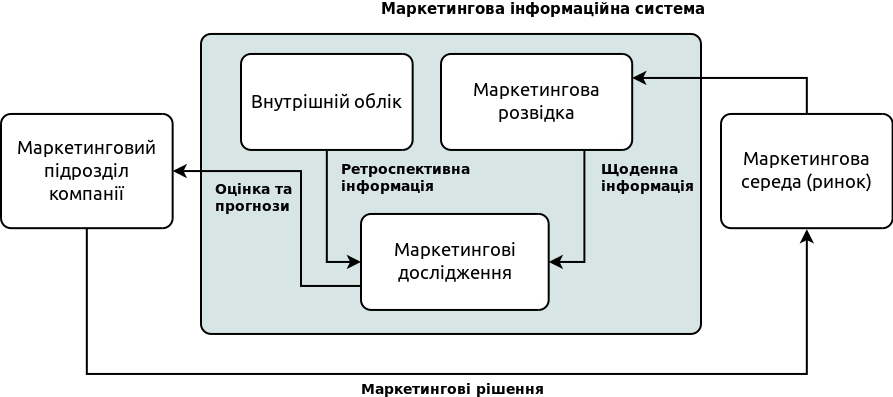
\includegraphics[width=7in]{images/mis_structure.png}
\caption{Структура МІС}
\label{fig:mis_structure}
\end{stdfigure}    

\subsubsection{Проблеми МІС}
%    MIS складається з трьох частин:
Маркетингова інформаційна система складається з трьох частин (див. рис. \ref{fig:mis_structure})\cite{kotler14}: 
\begin{itemize}
\item внутрішній облік (англ. {\it internal records});
\item маркетингові дослідження (англ. {\it marketing research});
\item маркетингова розвідка (англ. {\it marketing intelligence}).
\end{itemize}

В процессі визначення важливих можливостей та потенційних проблем, маркетологи покладаються внутрішню ретроспективну звітність компанії про замовлення, продажі, ціну, вартість, наявність товару тощо. Найважливішою частиною цієї звітності є інформація про цикл замовлення-розрахунок: розміщення замовлення, підготовка рахунків-фактур. Також, компанії ретельно збирають інформацію про клієнтів, їх вподобання, вік та т.і. Зазвичай, внутрішній облік реалізується системами класів ERP та CRM, що й визначає основні проблеми забезпечення збору звітності: інтеграція ERP та CRM систем, організація сховища даних тощо, потребують значних фінаносвих витрат та часу.
% Що це? Почему так важно? Що збираеться?
% Як збираэться? DH, CRM/ERP, OLTP. Проблеми: затраты ресурсов на организацию DH и сбора информации.

Система маркетингової розвідки --- це процедури та джерела, які використовують маркетологи для збору щоденної інформації про стан маркетингової середи\cite{kotler14}. Маркетологи збирають поточні дані за допомогою державних звітів, ЗМІ та інтернету, зворотнього зв’язку з клієнтами і посередниками. Інформація, що отримується в процесі маркетингової розвідки, обов’язково аналізується та є однією з основ для прийняття рішень про поведінку компанії на ринку в майбутньому.
% Це постійний збір інформації про ринок, клієнтів на конкурентів, що дозволяє прогнозувати ситуацію на ринку.
% Що це? Навыщо? Що збираэться? Ретроспектива, тренди
% Проблеми: нема перспективних данних для того, що робити прогнози
% TODO: слідити за числом слова "компанія"

На основні зібраних ретроспективних (системами внутрішнього обліка) та поточних даних (системами маркетингової розвідки) компанія проводить маркетингові дослідження. Результатом досліджень є оцінка маркетингових можливостей, що були використані та прогнозування можливостей, що можуть бути використані в майбутньому; оцінюються та прогнозуються, наприклад, розмір, прибутковість та потенціал можливостей. Точність результатів дослідження є дуже важливою, бо саме прогнозований об’єм продажів визначає об’єм виробництва, структуру каналу розповсюдження (або, маркетингового каналу), бюджет на рекламу тощо. Для забезпечення підтримки роботи аналітиків використовують OLAP-системи та засоби data mining, що дозволяють проводити різні види аналізу та шукати закономірності в даних.
% Нашо? Что делает? Пронозирует. На основе чего?
% На основні ретроспективни даних, що були зібрані системами внутрішнього обліку, аналітики роблять висновки про наявні результати, помилки, що були допущені. 
% Але найбільший інтерес викликають системи маетингової розвідки, за допомогою яких.
% TODO: OLAP в список позначень та скорочень
% TODO: схему в иллюстрации и слайди!
 

\subsubsection{Маркетингова розвідка}
% Що то? Нащо треба? несколько предложений
% TODO: схема, в которой отсутствует прогнозирование.
% Из каких частей состоит?
% Отсутствует перспектива. Предлагается использовать преспективу с помощью моделирования
% Пропонується моделювати маркетинговий канал (дати визначення) для того, що перспективну інформацію.

\subsubsection{Бізнес-ігри}
% кратко: що таке бізнес-ігри, бизнес-симуляция.
% Предлагаю автоматизировать. 

\subsection{Постановка задачі}
\subsubsection{Моделювання маркетингового каналу}
%TODO: що таке концепція маркетингового каналу, основні момент структури та керування каналом.
% TODO: постановка задачі моделювання ()

\subsubsection{Вимоги до програмного забезпечення}
 
